\documentclass[11pt]{article}
\usepackage[review]{acl}
\usepackage{times}
\usepackage[T1]{fontenc}
\usepackage[utf8]{inputenc}
\usepackage{microtype}
\usepackage{booktabs}
\usepackage{array}
\usepackage{graphicx}
\usepackage{xurl}
\newcommand{\code}[1]{\texttt{#1}}
\title{Methods of Finding Longer, Readable Palindromes}
\hypersetup{pdftitle={Methods of Finding Longer, Readable Palindromes}}
\hypersetup{pdfsubject={October 9 paper revision of public v1}}
\author{Anonymous submission}

\begin{document}
\maketitle

\begin{abstract}
We search for exact English palindromes of 30--119 letters and test whether penalizing recurring phrases improves the outputs. Across 360 matched runs, penalties 0, 4, and 16 each return 90 exact outputs from 120 attempts. Both penalties eliminate six targeted trigrams and increase distinct texts from 69 to 78. New fragments recur, however, and strict mechanical acceptance falls from 59/120 to 28/120. None of 148 distinct candidates passes a separate model's grammar-and-meaning threshold. This controlled comparison identifies a limitation of fragment penalties and provides frozen outputs and reproducible analysis. Human ratings remain uncollected.
\end{abstract}

\section{Introduction}
A palindrome reads identically forward and backward after removing spaces, punctuation, and case. For example, \emph{Never odd or even.} becomes \code{neveroddoreven}. Longer strings can satisfy this rule while lacking a clear sentence parse or meaning. Table~\ref{tab:illustrations} gives short readable illustrations; Table~\ref{tab:outputs} shows actual search outputs.

In a prior collection, 46/52 distinct outputs contained \emph{no it a}. We fixed the six most prevalent trigrams before running new seeds, then penalized their reuse under matched search limits. We measure exact-output yield, diversity, structural shortcuts, and model-rated language quality separately.

\begin{table}[t]
\centering
\small
\begin{tabular}{@{}p{.82\columnwidth}r@{}}
\toprule
Illustration and normalized letter stream & Letters \\
\midrule
\emph{No rider sees red iron.} & 18 \\
\code{noriderseesrediron} & \\[2pt]
\emph{Liam sees mail.} & 12 \\
\code{liamseesmail} & \\[2pt]
\emph{No evil did live on.} & 15 \\
\code{noevildidliveon} & \\
\bottomrule
\end{tabular}
\caption{Exact illustrative palindromes, verified after ASCII-letter normalization. These are calibration examples, not experimental discoveries or human-study results. The latter two are known-existing examples; novelty of the first is unverified.}
\label{tab:illustrations}
\end{table}

\paragraph{Related work.}
Palindrome generators match character sequences \citep{norvig2002palindrome} or search n-gram graphs \citep{papadopoulos2015palindromes}. \citet{bonlarron-regin-2024} combine constraints and language scores for RADNER sentences. We isolate a scoring intervention within two implementations. Evaluation research motivates testing metrics \citep{sai-etal-2021-perturbation} and defining quality dimensions \citep{howcroft-etal-2020-twenty}.

\section{Paired intervention}
\paragraph{Construction and search.}
A paired construction writes $L\,C\,R$, where the normalized $R$ reverses $L$ and $C$ is itself palindromic. In \emph{Liam sees mail.}, \code{liam} reverses to \code{mail}, and \code{sees} supplies the center. Word boundaries need not mirror: the same constraint can join differently segmented word sequences.

Both searches start from empty text using one frozen vocabulary filtered from a 30K word list. Outside-in search extends outer word sequences toward their meeting point, closing when the unmatched character residual is palindromic. Center-out search grows away from the center and closes on empty overhang. We compare penalties within each implementation; their native closure rules differ.

The baseline adds English Zipf word frequency \citep{speer-2022-wordfreq} and 0.3 per character, subtracts 2 per prior word use and 4 for adjacent repetition, and adds seeded perturbations for beam ranking. Final selection uses the unperturbed accumulated score per normalized letter.

\begin{figure*}[t]
\centering
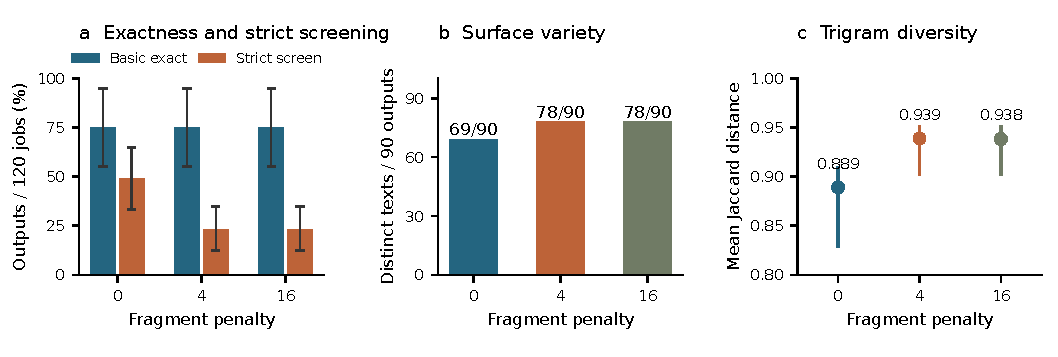
\includegraphics[width=\textwidth]{fig/fragment-penalty-tradeoff.pdf}
\caption{\textbf{More variety accompanies fewer strict passes.} Each arm receives 120 jobs: 20 shared seeds, three length bands, and two methods. (a) Basic exact coverage is 90/120 throughout; strict coverage is 59/120, 28/120, and 28/120. (b) Distinct surfaces among the 90 outputs. (c) Mean trigram-set Jaccard distance; higher means less overlap. Error bars in (a) and lines in (c) show 95\% paired seed-bootstrap intervals. Distinct counts have no interval.}
\label{fig:tradeoff}
\end{figure*}

\paragraph{Admission and screening.}
The basic gate requires ASCII rendering, exact letter reversal, the requested length, lexicon membership, an allowlist for words of at most two letters, and exclusions for listed catalogue examples and templates. Repeated words are allowed. After selection, a strict screen also rejects repeated content words, self-palindromic content words, proper palindromic multiword spans, repeated units containing content words, and boundary-aligned word reversals. It does not rerun search. Both coverages use all requested jobs as their denominator. The strict screen measures structural restrictions, not readability: it would reject \emph{Liam sees mail.} for its center word \emph{sees}.

\paragraph{Frozen penalty.}
The targets are \emph{no it a}, \emph{a i cos}, \emph{it a i}, \emph{cos same open}, \emph{i cos same}, and \emph{one poem association}. We rank trigrams by the number of prior distinct texts containing them, breaking ties alphabetically. Let $F(x)$ count their occurrences, including overlaps, in the current concatenated word sequence. For parent $x$ and child $x'$, the score increment becomes
\begin{equation}
\Delta S_\lambda=\Delta S-\lambda\bigl[F(x')-F(x)\bigr].
\end{equation}
These changes sum to $-\lambda F(x)$ at closure and refund a penalty when growth breaks a temporary join. Strengths $\lambda\in\{0,4,16\}$ were fixed before the new outputs and ratings. Only ranking and selection scores change.

\paragraph{Matched tasks.}
Twenty fresh seeds (7100--7119), three letter bands (30--49, 50--79, 80--119), two methods, and three strengths yield 360 jobs. Each seed--band--method block executes all strengths on one worker in seeded random order. Every job receives beam width 256, candidate limit 800, per-parent limit 32, at most 400 steps, 32 words, 24 residual letters, and 180 seconds. Appendix~\ref{sec:implementation} gives execution details.

\section{Measurements}
\paragraph{Diversity and uncertainty.}
Lexical analyses collapse identical surfaces within each arm and tokenize lowercase ASCII words. Trigram-set distance is $1-|A\cap B|/|A\cup B|$, averaged over all unordered pairs of distinct texts. We also count targeted-fragment occurrences and the prevalence of every trigram (Figure~\ref{fig:motifs}).

We use 20,000 paired percentile bootstrap replicates, resampling 20 seeds while retaining their methods, bands, and arms together (PRNG seed 20261002). Diversity is recomputed after duplicate collapse in each resample. This measures search-seed variability on the fixed vocabulary; pairwise text comparisons are not independent trials. We report both strengths against baseline. Raw distinct counts receive no interval because resampling observed strings biases richness downward.

\begin{figure*}[t]
\centering
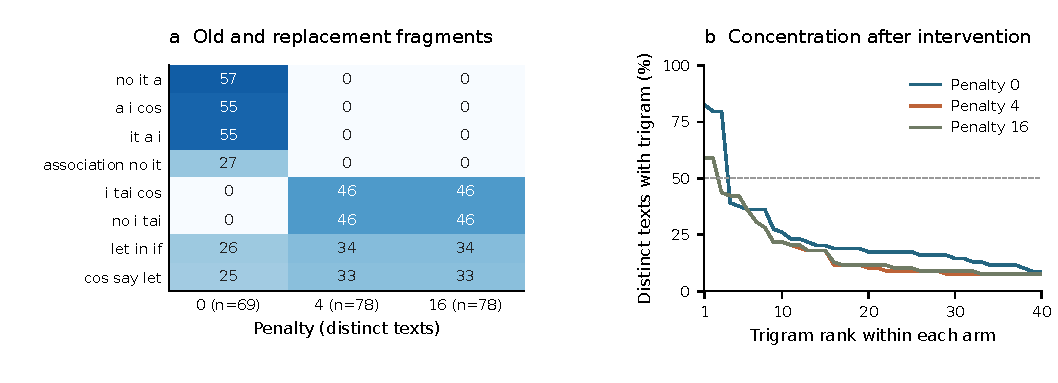
\includegraphics[width=\textwidth]{fig/fragment-penalty-motifs.pdf}
\caption{\textbf{Replacement fragments remain concentrated.} (a) Counts of distinct texts containing each trigram, with arm denominators beneath the columns. Rows are the union of the four most prevalent trigrams at penalties 0 and 4, ranked by count with alphabetical ties within each arm. Color shows the proportion. (b) Prevalence of each arm's 40 highest-ranked trigrams. The maximum falls from 57/69 (82.6\%) to 46/78 (59.0\%). Overlapping trigrams are counted separately. All six targets are absent from both penalized arms.}
\label{fig:motifs}
\end{figure*}

\paragraph{Blinded model audit.}
Qwen3 32B on Bedrock \citep{awsbedrockqwen332b} rates grammaticality and coherent meaning from 0 to 3, seeing exact text without method or penalty labels. A joint pass requires both scores $\geq2$. The control gate requires at least 8/12 held-out Brown prose controls \citep{kucera-francis-1967} and at most 3/12 corresponding shuffles to pass. All 148 distinct candidates are rated once; shared texts reuse that rating. Twelve hidden repeats check consistency. Appendix~\ref{sec:rubric} gives anchors and presentation details.

\section{Results}
\paragraph{Exactness and diversity.}
All arms return 90/120 exact outputs, succeeding on the same tasks with 15/20 in every method--band cell. Distinct surfaces rise from 69 to 78. At penalty 4, mean trigram distance increases from 0.889 to 0.939 (paired difference $+0.050$, 95\% interval $[0.026,0.087]$), and maximum trigram prevalence falls by 23.6 percentage points ($[-37.2,-7.9]$). Penalty 16 yields 78 surfaces and distance 0.938; its text differs from penalty 4 on eight tasks (Figure~\ref{fig:tradeoff}).

\paragraph{Repetition and shortcuts.}
Both penalties remove all targets from all 90 selected outputs, but \emph{i tai cos} and \emph{no i tai} each occur in 46/78 distinct penalized texts. Strict coverage drops from 59/120 to 28/120, a difference of $-25.8$ percentage points ($[-37.5,-15.0]$). Figure~\ref{fig:strata} locates the loss across methods and bands. Self-palindromic proper spans occur in 21/90 baseline outputs, 58/90 at penalty 4, and 61/90 at penalty 16; self-palindromic words occur in 17/90, 16/90, and 16/90. These failure counts overlap.

\begin{figure}[t]
\centering
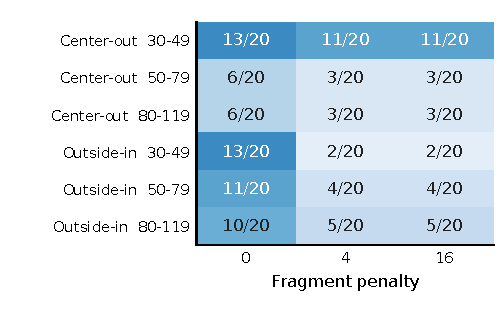
\includegraphics[width=\columnwidth]{fig/strict-screen-strata.pdf}
\caption{Strict passes among 20 requested jobs in each method--length cell. Every cell has 15 basic exact outputs. Color encodes the strict-pass fraction; counts retain failed jobs in the denominator. These are mechanical checks.}
\label{fig:strata}
\end{figure}

\begin{table}[t]
\centering
\footnotesize
\begin{tabular}{@{}p{\columnwidth}@{}}
\toprule
Baseline ($\lambda=0$) \\
\emph{In as if one poem association\newline no it a i cos same open of is an i.} \\[3pt]
Penalty 4 \\
\emph{At i definitely association no i tai cos say let in if edit a.} \\
\bottomrule
\end{tabular}
\caption{Selected outputs for the same seed (7100), method (center-out), and band (30--49). Each has 48 normalized letters, is exactly palindromic, passes the strict screen, and receives model scores $(0,0)$. The replacement fragment is visible in the second text. Full letter streams and record IDs appear in Appendix~\ref{sec:examples}.}
\label{tab:outputs}
\end{table}

\paragraph{Grammar and meaning.}
Qwen passes 11/12 prose controls and 0/12 shuffles. Of 148 distinct candidates, 142 receive $(0,0)$, three $(1,0)$, and three $(1,1)$ (Figure~\ref{fig:ratings}); none passes jointly. All 12 hidden repeats agree. Table~\ref{tab:outputs} illustrates that even strict passes can have no recoverable sentence parse under the rubric.

\begin{figure}[t]
\centering
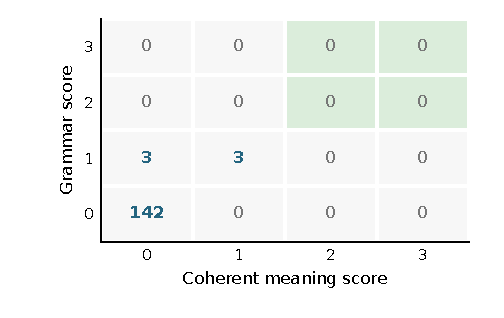
\includegraphics[width=\columnwidth]{fig/model-score-distribution.pdf}
\caption{Saved model scores for 148 distinct candidates pooled across arms. Cell entries count texts; shared outputs are counted once. The green quadrant requires both scores $\geq2$ and contains 0/148 candidates. Controls and hidden repeats are excluded.}
\label{fig:ratings}
\end{figure}

\section{Discussion and conclusion}
Fragment penalties preserve exact yield and improve surface variety, but redirect recurrence toward new fragments and select more structural shortcuts. Untargeted recurrence and post-selection screening expose effects that a targeted-fragment count misses. A human study with explicit dimensions and quality checks \citep{khashabi-etal-2022-genie} is needed to assess reader quality. Future work could score sentence structure and meaning during search.

\paragraph{Reproducibility.}
Frozen records, protocols, model responses, and analysis are supplied. The source bundle regenerates four figures and checks every example. Brown text is omitted.

\section*{Limitations}
The targets were chosen from inspected development outputs. Fresh seeds test one vocabulary and search family, with different native closure rules; there is no matched external-generator comparison. Diversity conditions on success, and duplicate collapse leaves shared-fragment dependence. Intervals use only 20 seed clusters and do not quantify uncertainty over languages, tasks, or readers. Identical paired yields and near-floor ratings do not establish population equivalence. The strict screen can reject readable examples. Qwen's small prose/shuffle control gate is not human or palindrome-domain calibration, and pretraining exposure to Brown is unknown. Hosted inference exposes neither a provider seed nor a weight digest. No human ratings were collected, and illustrative examples establish no discovery or readable-length record.

\section*{Ethical considerations}
No participant data were collected. Generative AI assisted implementation, writing, and review.

\bibliography{refs}
\appendix
\newpage
\section{Search implementation and execution}\label{sec:implementation}
The baseline uses \code{wordfreq} 3.1.1. Seeded uniform perturbations in $[0,0.4)$ affect child priorities but not accumulated closure scores. Exhaustive toy tests of both growth directions verify penalty increments against full-sequence counts, including refunds for broken joins. At strength zero the wrapper returns the baseline score unchanged.

All 360 jobs completed without execution errors or deadlines on 32 workers of an AWS c7i.16xlarge CPU instance (64 virtual CPUs). Mean elapsed times were 2.96, 3.04, and 3.03 seconds; mean scorer-call counts were 56,415, 52,679, and 52,722 for penalties 0, 4, and 16. Scorer calls count evaluated word extensions. Equal limits do not guarantee equal expansions. Both gates, failed jobs, and timings are retained.

\section{Model rubric and controls}\label{sec:rubric}
The model is \code{qwen.qwen3-32b-v1:0}, using temperature 0, top-p 1, maximum 128 output tokens, a no-thinking directive, and structured JSON. It assesses exact text without repair or rewards for symmetry.

Grammar anchors are: 0, no recoverable sentence parse; 1, isolated grammatical phrases with major sentence breaks; 2, a mostly recoverable but strained parse; 3, natural grammatical connected English. Meaning anchors are: 0, no recoverable proposition or event; 1, word associations with unclear relations; 2, a plausible but incomplete or vague interpretation; 3, clear meaning with understandable relations.

The prose and shuffle controls reuse the prior audit's hash-verified Brown spans; seven prose controls have multiple sentences. The 148 candidates and 12 repeats follow a fixed hash-derived order after the control gate. Repeats contain six candidates and six prose controls selected by ascending hash. The inventory was fixed after generation and before judge calls; the rubric and thresholds predate generation. Only exact text and rubric enter model messages. Ratings do not affect search or selection.

\newpage
\section{Example verification}\label{sec:examples}
Every example is checked by retaining lowercase ASCII letters and comparing the resulting stream with its reverse. Table~\ref{tab:illustrations} gives three streams; \emph{Never odd or even.} has 14 letters. The readable examples are illustrative calibration material, with provenance recorded in the source bundle.

The first experimental example is record \code{s7100-b1-center-p0}, normalized as
\begin{quote}\small\ttfamily
inasifonepoemassociation\\
noitaicossameopenofisani
\end{quote}
The second is \code{s7100-b1-center-p4}, normalized as
\begin{quote}\small\ttfamily
atidefinitelyassociation\\
noitaicossayletinifedita
\end{quote}
Line breaks are display-only: each concatenation has 48 letters and equals its reverse. Both texts pass the saved strict screen and receive grammar and meaning scores of zero.

\section{Development evidence}
The targets come from 52 distinct texts in an earlier 240-job resource comparison, separate from the 360-job intervention. A later 32-job development sweep uses two new seeds, both methods, bands 120--159 and 800--999, a 256-word cap, and penalties 0, 1, 2, and 4. Each arm returns 4/8 exact outputs; 0/16 selected outputs pass the strict screen. The longest has 824 letters and no readability ratings. These exploratory results establish neither an optimal penalty nor a readable-length gain.

\section{Offline reproduction}
The source bundle includes frozen record copies, their source hashes, the paired bootstrap analysis, and a figure builder. Running \code{python3 revision/build\_figures.py} from the paper directory verifies record and text hashes, parses saved judge responses, reproduces all four vector figures, and checks every example. The original evidence archive retains the search implementation and protocols.
\end{document}
